\documentclass[a4paper, 11pt]{article}
    \usepackage[left=2cm, top=3cm, text={17cm,24cm}]{geometry}
    \usepackage[utf8]{inputenc}
    \usepackage[T1]{fontenc}
    \usepackage{times}
    \usepackage{graphics}
    \usepackage{subcaption}
    \usepackage{hyperref}

\begin{document}

\begin{titlepage}
    \begin{center}
        \textsc{\Huge{Brno University of Technology\\[0.4em]}
        \huge{Faculty of Information Technology}}\\        
        \vspace{\stretch{0.382}}
        \huge{\textbf{Documentation of compiler for language \textsc{IFJ24}}}\\
        \LARGE{Team xnovakf00\,--\,variant vv-BVS}\\
        \Large{extensions: \textsc{funexp}}\\
        \vspace{\stretch{0.618}}
    \end{center}
    \Large{Matúš Fignár xfignam00\,--\,25\%\\
            Tibor Malega xmalegt00\,--\,25\%\\
            Filip Novák xnovakf00\,--\,team leader\,--\,25\%\\
            Ján Skovajsa xskovaj00\,--\,25\%\hfill \today}
\end{titlepage}

\tableofcontents
\newpage
\listoffigures
\newpage

% ODTADE PISTE CO CHCETE, KED CHCETE ODSEK POUZITE \section{NAZOV}, KED PODODSEK \subsection{NAZOV},
% ESTE MENSI TA \subsubsection....
% KOMENTARE CEZ %

% KED KOD/NIECO TECHNICKE tak \verb | TEXT |
% KED VSETKO VELKYM (AKO NAPR FUNEXP NA TITULKE) TAK \textsc{TEXT}
% HRUBE \textbf{TEXT}
% ITALICS \textit{TEXT}
% KEBY HOCICO INE POTREBUJETE TAK TAG ME

\section{Design and implementation of the compiler}
Compiler uses double-traversal method of the source code based on "top-down" recursive parsing specified by
LL1 grammar\footnote{See figures \ref{ll1rules} and \ref{ll1table}.}. Expressions are processed using precedence syntactic
analysis. Lexical analyser (scanner) processes source code and tokenizes it based on deterministic finite automaton\footnote{See figure \ref{automaton}.}.
During parsing, semantic analysis is performed and abstract syntactic tree (AST) is constructed for internal representation.
Compiler uses table of symbols (symtable), implemented as height-balanced binary search tree for keeping information about defined functions and variables.
Code is generated through recursive traversal of constructed AST.

\section{Lexical analysis}

\section{Syntactic analysis}
Syntactic analysis is divided into two parts\,--\,expression parser (found in \verb|expression_parser.c, expression_parser.h|) and
recursive parser processing the rest of the source code (found in \verb|parser.c, parser.h|). These two are closely entertwined.
Both call scanner to receive tokens to evaluate.\par
When recursive parser expects an expression in source code (denoted as \verb|expression| in LL1 grammar~(\ref{ll1rules})), 
expression parser is called for processing.
\subsection{"Top-down" syntactic analysis}

\subsection{"Bottom-up" syntactic analysis of expressions}

\section{Semantic analysis}

\section{Table of symbols}

\section{Abstract syntactic tree}
Abstract syntactic tree (found in \verb|ast.c, ast.h|) is implemented as acyclic graph with specialised nodes.
Based on the type of a node, different information is stored and number of child nodes varies as well.
\section{Code generation}

\section{Teamwork}
Implementing a compiler is not an easy task, that is why the work has begun as soon as 
the assignment was published. Firstly, tasks were distributed among all members based on 
preferences.\par 
Test submission was set as deadline for implementation. This deadline
was successfuly met with time left for fixing errors and further testing. Pair programming as well as 
code reviews were practised. 

\subsection{Communication}
Discord was chosen as primary mean of communication. In specialised voice and text channels meetings were
held at least once a week. Git was used as versioning system with remote repository hosted by team leader at
GitHub. Using webhook, Discord bot for notifications about changes on remote repository was added.\par
Email addresses and telephone numbers were shared among all members in case of an unexpected situation.
Luckily, no problems were encountered and communication ran smoothly for the whole duration of the project.

\subsection{Task distribution}
\begin{itemize}

    \item \textbf{Matúš Fignár xfignam00}\,--\,precedence table, "bottom-up" expression parsing
    \item \textbf{Tibor Malega xmalegt00}\,--\,finite automaton design, lexical analysis
    \item \textbf{Filip Novák xnovakf00}\,--\,"top-down" recursive parsing, table of symbols
    \item \textbf{Ján Skovajsa xskovaj00}\,--\,code generation, testing

\end{itemize}
The remaining parts of the project were developed by all members of the team simultaneously.















\section{Attachments}
\begin{figure}[ht]
    \begin{center}
        \scalebox{0.25}{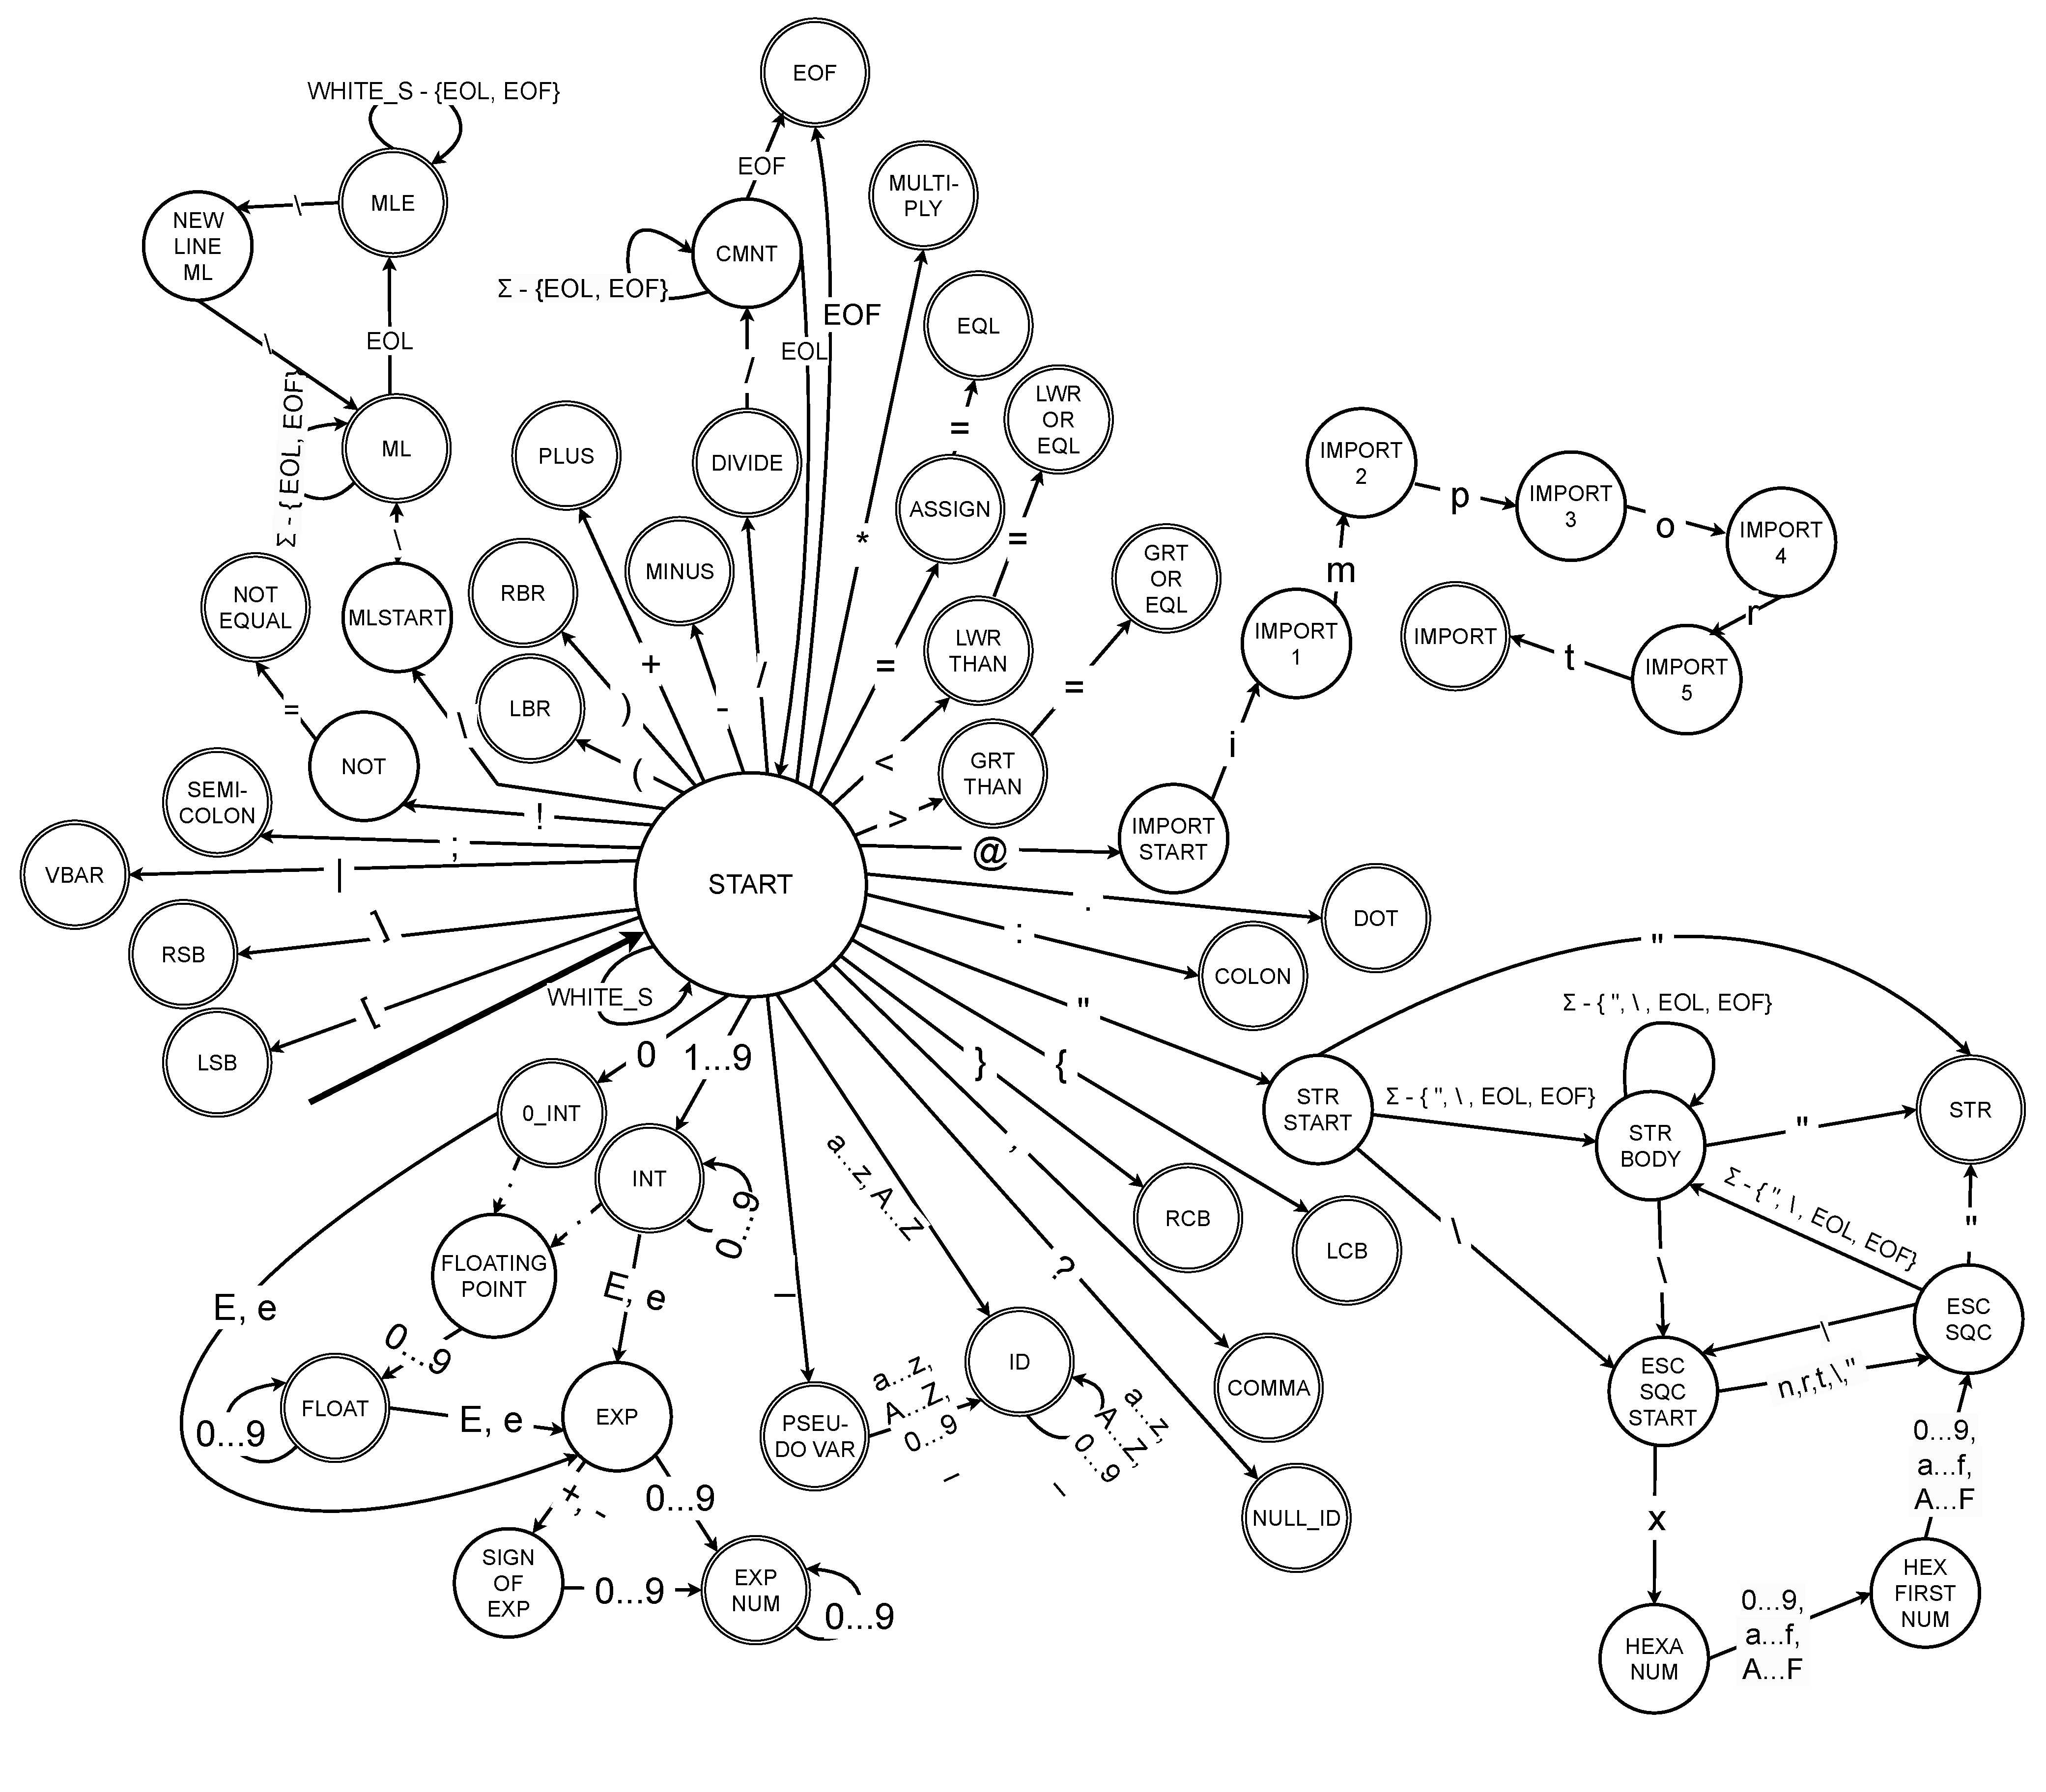
\includegraphics{doc/automaton.pdf}}
        \caption{Deterministic finite automaton for lexical analysis}
        \label{automaton}
    \end{center}
\end{figure}

\begin{figure}[ht]
    \begin{center}
    \begin{enumerate}
        \itemsep-0.5em
        \item \textless prog\textgreater\  $\to$ \textless prolog\textgreater\ \textless code\textgreater
        \item \textless prolog\textgreater\ $\to$ const id = @import ( expression ) ;
        \item \textless code\textgreater\ $\to$ \textless def\_func\textgreater\ \textless code\textgreater
        \item \textless code\textgreater\ $\to$ $\varepsilon$
        \item \textless def\_func\textgreater\ $\to$ pub fn id ( \textless params\textgreater ) \textless type\_func\_ret\textgreater\ \{ \textless body\textgreater \}
        \item \textless params\textgreater\ $\to$ id : \textless type\textgreater\ \textless params\_n\textgreater
        \item \textless params\textgreater\ $\to$ $\varepsilon$
        \item \textless params\_n\textgreater\ $\to$ , \textless params\textgreater
        \item \textless params\_n\textgreater\ $\to$ $\varepsilon$
        \item \textless def\_variable\textgreater\ $\to$ \textless varorconst\textgreater\ id \textless type\_var\_def\textgreater\ = expression ;
        \item \textless varorconst\textgreater\ $\to$ const
        \item \textless varorconst\textgreater\ $\to$ var
        \item \textless unused\_decl\textgreater\ $\to$ \_ = expression ;
        \item \textless type\_normal\textgreater\ $\to$ i32
        \item \textless type\_normal\textgreater\ $\to$ f64
        \item \textless type\_normal\textgreater\ $\to$ [ ] u8
        \item \textless type\_null\textgreater\ $\to$ ? \textless type\_normal\textgreater
        \item \textless type\textgreater\ $\to$ \textless type\_normal\textgreater
        \item \textless type\textgreater\ $\to$ \textless type\_null\textgreater
        \item \textless type\_func\_ret\textgreater\ $\to$ \textless type\textgreater
        \item \textless type\_func\_ret\textgreater\ $\to$ void
        \item \textless type\_var\_def\textgreater\ $\to$ : \textless type\textgreater
        \item \textless type\_var\_def\textgreater\ $\to$ $\varepsilon$
        \item \textless expr\_params\textgreater\ $\to$ expression \textless expr\_params\_n\textgreater
        \item \textless expr\_params\textgreater\ $\to$ $\varepsilon$
        \item \textless expr\_params\_n\textgreater\ $\to$ , \textless expr\_params\textgreater
        \item \textless expr\_params\_n\textgreater\ $\to$ $\varepsilon$
        \item \textless after\_id\textgreater\ $\to$ = expression ;
        \item \textless after\_id\textgreater\ $\to$ \textless builtin\textgreater\ ( \textless expr\_params\textgreater ) ;
        \item \textless assign\_or\_f\_call\textgreater\ $\to$ id \textless after\_id\textgreater
        \item \textless builtin\textgreater\ $\to$ . id
        \item \textless builtin\textgreater\ $\to$ $\varepsilon$
        \item \textless st\textgreater\ $\to$ \textless def\_variable\textgreater
        \item \textless st\textgreater\ $\to$ \textless assign\_or\_f\_call\textgreater
        \item \textless st\textgreater\ $\to$ \textless unused\_decl\textgreater
        \item \textless st\textgreater\ $\to$ \textless while\_statement\textgreater
        \item \textless st\textgreater\ $\to$ \textless if\_statement\textgreater
        \item \textless st\textgreater\ $\to$ \textless return\textgreater
        \item \textless body\textgreater\ $\to$ $\varepsilon$
        \item \textless body\textgreater\ $\to$ \textless st\textgreater\ \textless body\textgreater
        \item \textless return\textgreater\ $\to$ return \textless exp\_func\_ret\textgreater  ;
        \item \textless exp\_func\_ret\textgreater\ $\to$ $\varepsilon$
        \item \textless exp\_func\_ret\textgreater\ $\to$ expression
        \item \textless id\_without\_null\textgreater\ $\to$ | id |
        \item \textless id\_without\_null\textgreater\ $\to$ $\varepsilon$
        \item \textless while\_statement\textgreater\ $\to$ while ( expression ) \textless id\_without\_null\textgreater\ \{ \textless body\textgreater \}
        \item \textless if\_statement\textgreater\ $\to$ if ( expression ) \textless id\_without\_null\textgreater\ \{ \textless body\textgreater \} else \{ \textless body\textgreater \}
    \end{enumerate}
    \caption{LL1 rules}
    \label{ll1rules}
\end{center}
\end{figure}

\begin{figure}[ht]
    \begin{center}
        \scalebox{0.7}{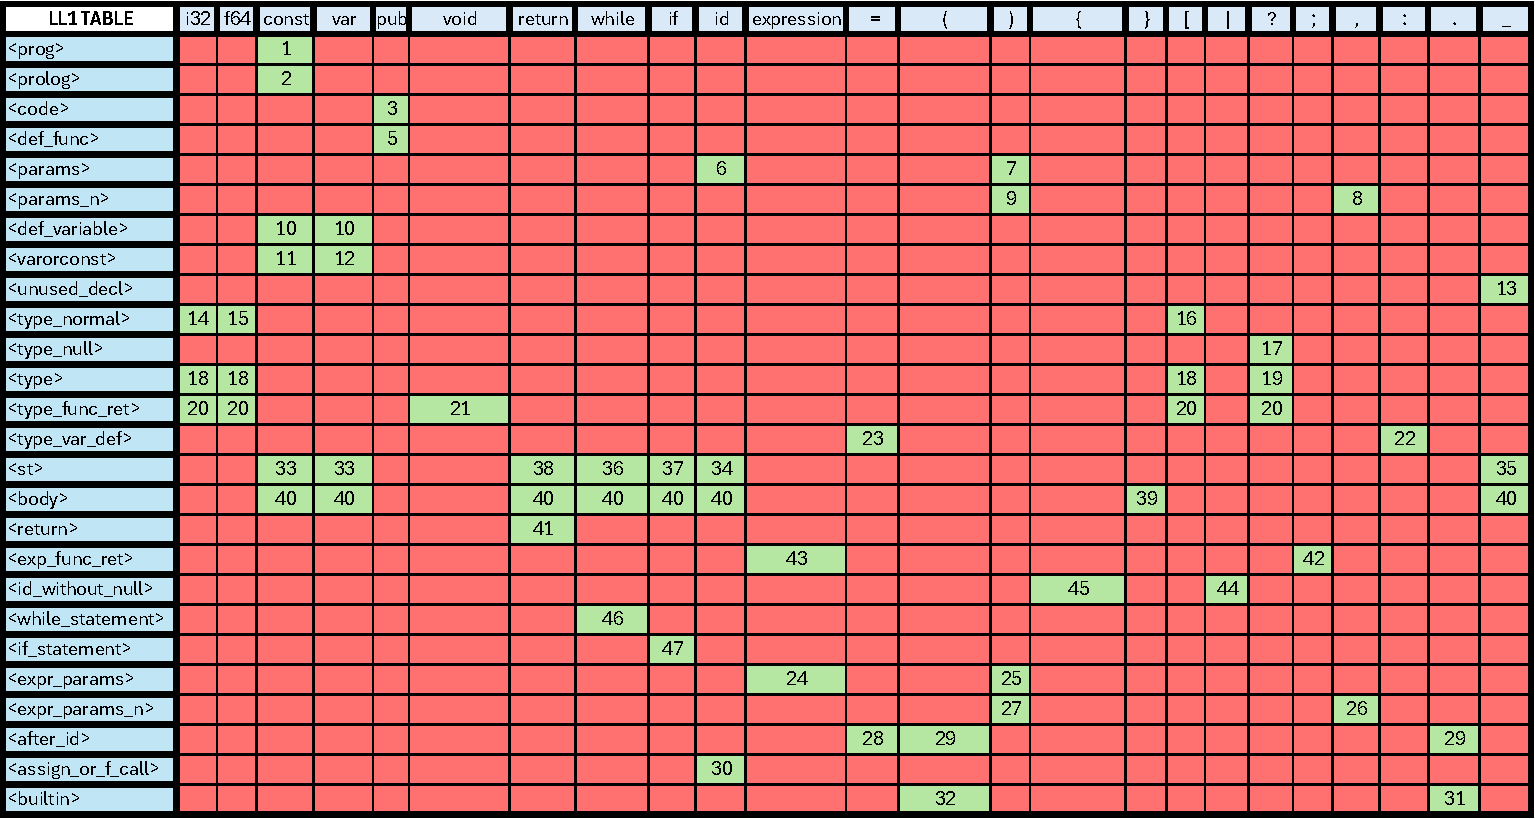
\includegraphics{doc/LL1_table.pdf}}
        \caption{LL1 table for parsing}
        \label{ll1table}
    \end{center}
\end{figure}

\end{document}